\chapter{EXPERIMENTAL METHODS} \label{ch:experiment}

\section{Optical Properties}
\subsection{Absorption Coefficients}
\subsection{Scattering Coefficients}
\subsection{Volume Scattering Function}

\section{Frond Distribution Parameters}
\subsection{Rotation}
\subsection{Lift}

\section{Current Progress: Experimental Data Analysis}

\subsection{Experimental Setup}
Thus far, besides beginning to study literature on the subject, I have been analyzing data collected from an experiment that Dr. Rogers and his colleagues performed several weeks ago in the sea near Trondheim to measure attenuation with and without the influence of kelp shading. The experimental setup was as follows. A rope is attached to a buoy and allowed to hang freely in the water. Fixed to the rope are light sensors spaced 1m apart from one another from 1m below the water's surface to 8m. Samples are collected simultaneously from all sensors every 10 seconds for several hours. A second such rope is placed nearby in the water during the same time, but with one kelp plant attached to it. Similar measurements are taken. After a certain time, a second kelp plant is attached to the rope. Similar measurements are taken once again.

\subsection{Data and Model}
I was given raw data from the sensors separated into one text file for each light sensor, each containing many lines with the time and intensity of the individual measurements. I have used Python to perform some analysis on the data collected during the previously described experiment, and generate plots to visualize the data. I divided the raw data into 3 datasets:
\begin{itemize}
	\item \textbf{Control}: first rope without kelp,
	\item \textbf{1 Kelp}: second rope with one kelp plant
	\item \textbf{2 Kelp}: second rope with two kelp plants
\end{itemize}

Note that these datasets are not the same length. The sensors on the first rope were collecting data for a significantly longer period of time which encompassed the time periods when the other two datasets were being collected, as shown in the time plots below.

For each dataset, we sought to calculate the light attenuation according to the model:

\begin{equation}
	I(z) = I_0e^{-kz}
	\label{atten}
\end{equation}

where $I_0$ is the intensity of light on the surface of the water, and $k$ is the attenuation coefficient.

\pagebreak
\subsection{Regression Technique}
By doing exponential regression, these two parameters, $I_0$ and $k$ can be calculated. Notice that light is not actually being collected at the surface of the water, rather it is inferred based on the measurements at other depths.

These parameters can be calculated at each point in time in each dataset. This is done by converting the exponential model to a linear model by taking the logarithm of equation \ref{atten}, which gives

\begin{equation}
	\ln I(z) = \ln I_0 - kz
	\label{log_atten}
\end{equation}

Then, a simple least squares fit can be calculated by minimizing the sum, $R(k,I_0)$ of the squared differences between our linear model and the logarithm of the data points, given by the following function of our fit parameters.

\begin{equation}
	R(k,I_0) = \sum_{n=1}^N (\ln I_n - \ln I_0 + kz)^2
	\label{resid}
\end{equation}

where $z_n$ are the depths at which light is collected (i.e. 1m - 8m), $I_n$ are the measured intensities, and $N$ is the number of depths (i.e. 8). Let $R(k,I_0)$ be called the residual for the time step at we are performing the fitting. By taking partial derivatives with respect to both fit parameters, the residual can be minimized, producing the ideal fit (according to this definition of the residuals). Setting both derivatives to 0, we get the following matrix system of equations.

% Define x and y as used in this least squares fit
\newcommand\xls{z_n}
\newcommand\yls{\ln I_n}
\begin{equation}
	%\renewcommand\arraystretch{3}
	\begin{bmatrix}
		\sum_{n=1}^N \xls^2 & \sum_{n=1}^N \xls \\
		\sum_{n=1}^N \xls   & N \\
	\end{bmatrix}
%
	\begin{bmatrix}
		k \\
		I_0
	\end{bmatrix}
%
	=
%
	\begin{bmatrix}
		\sum_{n=1}^N \xls\yls \\
		\sum_{n=1}^N \yls \\
	\end{bmatrix}
	\label{lstsq}
\end{equation}

\subsection{Statistical Analysis}
\label{stats}
For each dataset, the previously described regression can be performed for each time step. This gives as many values of the fit parameters for the dataset as there are time steps. The mean ($\mu$) and standard deviation ($\sigma$) are given for both parameters for each dataset. Statistical description is also given of the $R^2$ values and of the raw intensity measurements (at all depths). \\

\begin{table}[H]
	\centering
	\begin{tabular}{lrrrr}
		\toprule
		&  $k$ & $I_0$ & Residuals & Intensity\\
		\midrule
		$\mu$ & 0.27 & 3.6+04 & 2.2e+09 & 1e+04 \\
		$\sigma$ & 0.046 & 2.7e+04 & 4.5e+09 & 1.3e+04 \\
	\end{tabular}
	\caption{Statistical info for \textbf{Control}}
	\label{stats_control}
\end{table}

\begin{table}[H]
	\centering
	\begin{tabular}{lrrrr}
		\toprule
		&  $k$ & $I_0$ & Residuals & Intensity\\
		\midrule
		$\mu$ & 0.34 & 5.6e+03 & 1.5e+09 & 2.2e+03 \\
		$\sigma$ & 0.25 & 2.1e+04 & 6.7e+09 & 1.3e+04 \\
	\end{tabular}
	\caption{Statistical info for \textbf{1 Kelp}}
	\label{stats_1_kelp}
\end{table}

\begin{table}[H]
	\centering
	\begin{tabular}{lrrrr}
		\toprule
		&  $k$ & $I_0$ & Residuals & Intensity\\
		\midrule
		$\mu$ & -0.65 & 3.4 & 2.9e+05 & 95 \\
		$\sigma$ & 0.12 & 4.3 & 5.2e+05 & 1.7e+02 \\
	\end{tabular}
	\caption{Statistical info for \textbf{2 Kelp}}
	\label{stats_2_kelp}
\end{table}
	
\pagebreak
\subsection{Visualization}
Several different visualization techniques are implemented below for the experimental data and for the fitted parameters

\subsubsection{Raw Data}

Light intensity is plotted over time for each of the 3 datasets. Each sensor is represented as a separate line.

\begin{figure}[H]
	\centering
	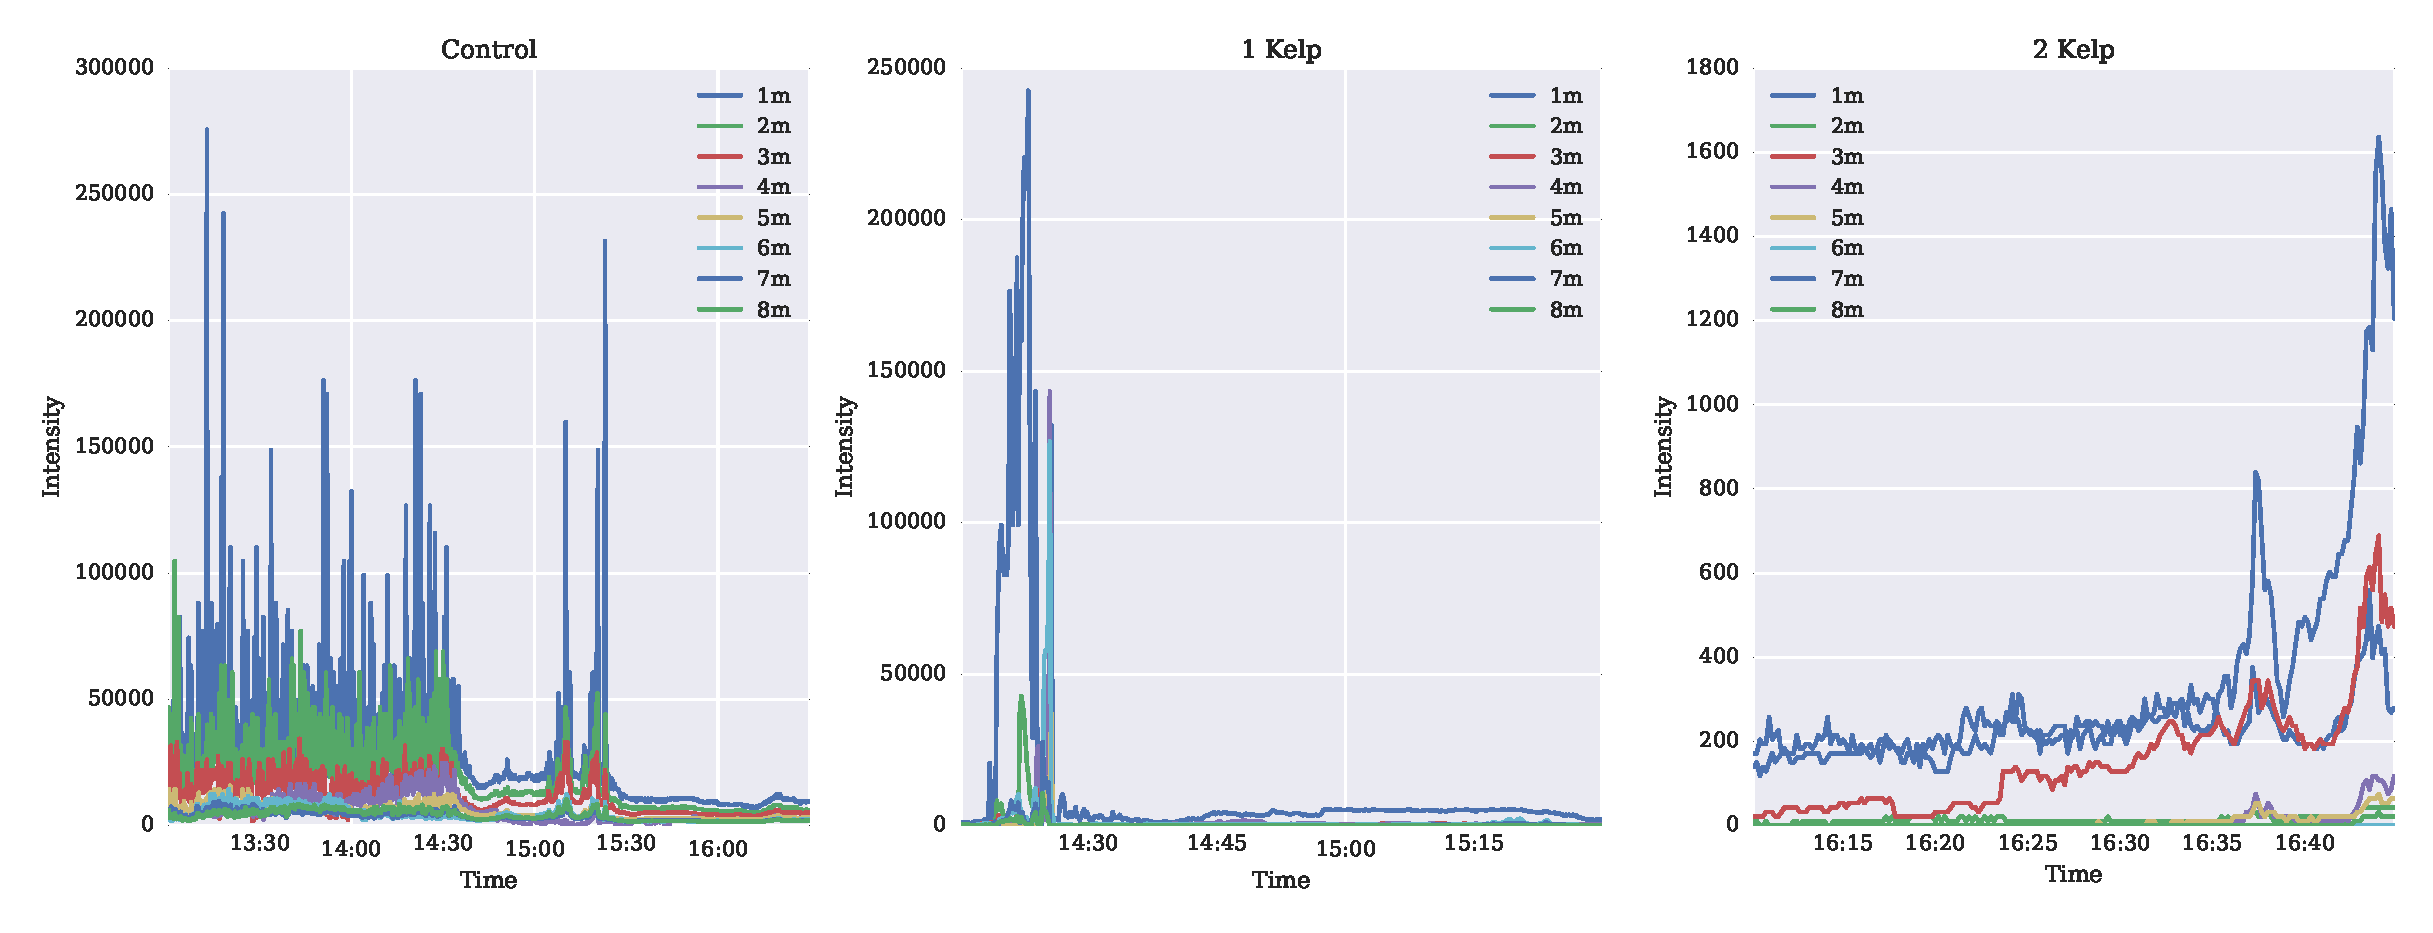
\includegraphics[width=\textwidth]{light_data.eps}
	\caption{Raw data: regular scale}
\end{figure}

\begin{figure}[H]
	\centering
	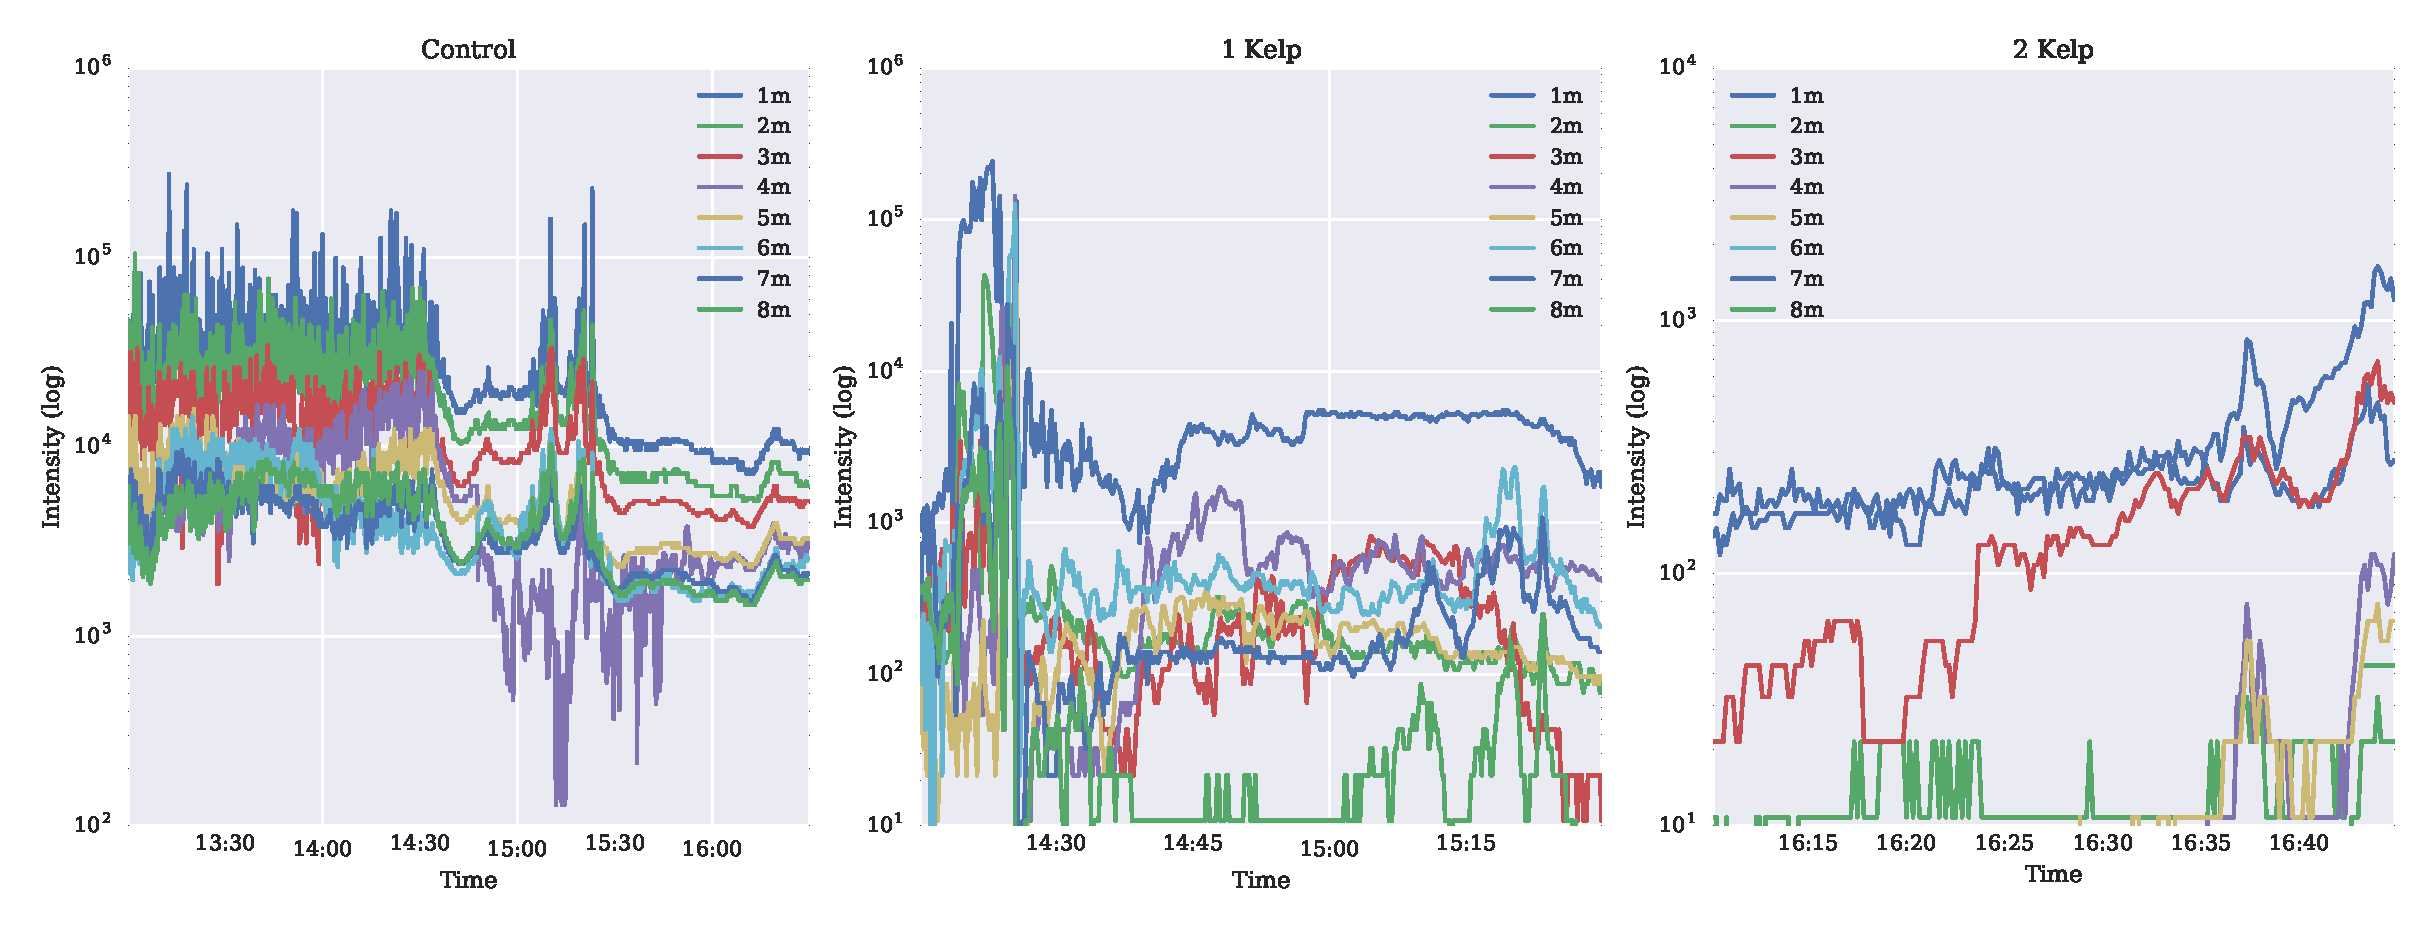
\includegraphics[width=\textwidth]{light_data_log.eps}
	\caption{Raw data: log scale}
\end{figure}

\pagebreak
\subsubsection{Parameters over time}
The fitted parameters are plotted over time. $R^2$ values are also plotted.

\begin{figure}[H]
	\centering
	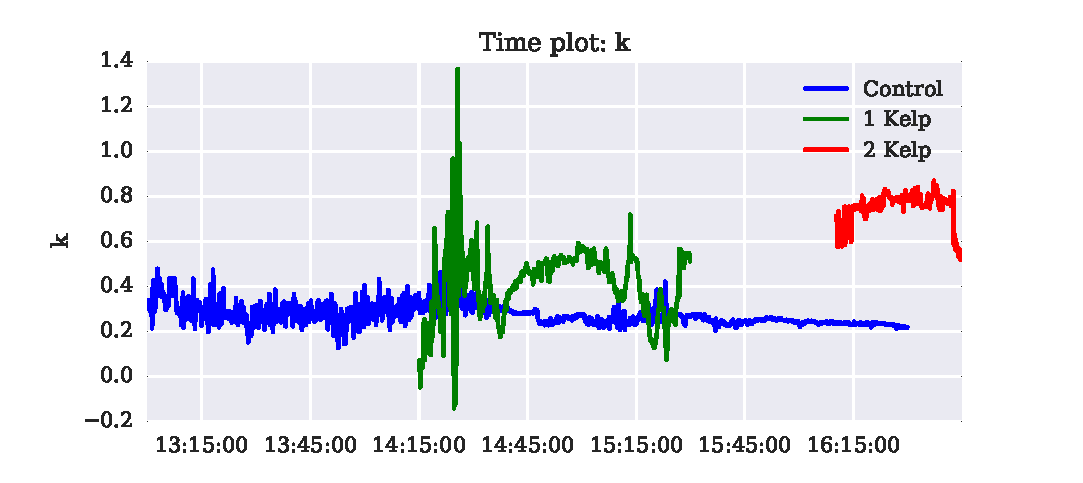
\includegraphics[width=\plotwidth]{time_k.eps}
	\caption{$k$ over time}
	\label{time_k}
\end{figure}

\begin{figure}[H]
	\centering
	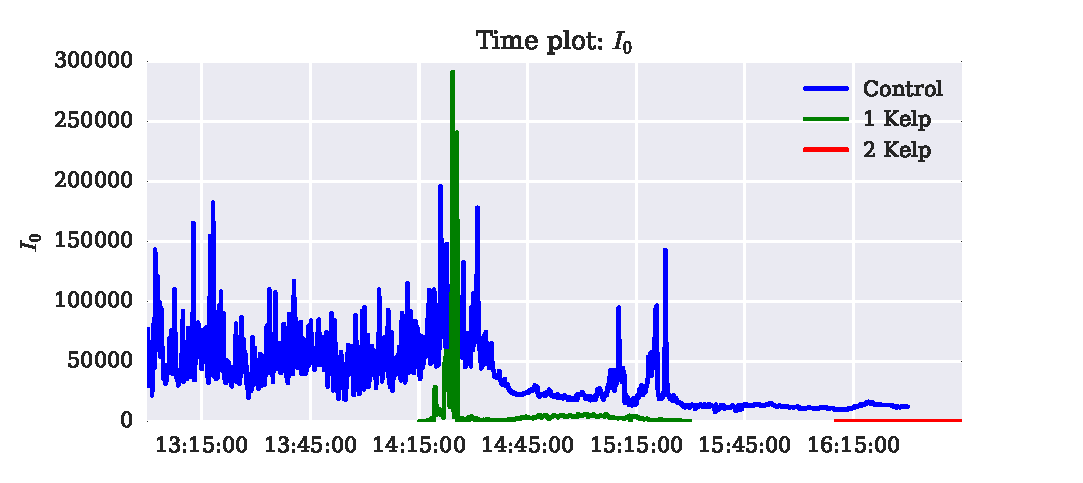
\includegraphics[width=\plotwidth]{time_I0.eps}
	\caption{$I_0$ over time}
	\label{time_I0}
\end{figure}

\begin{figure}[H]
	\centering
	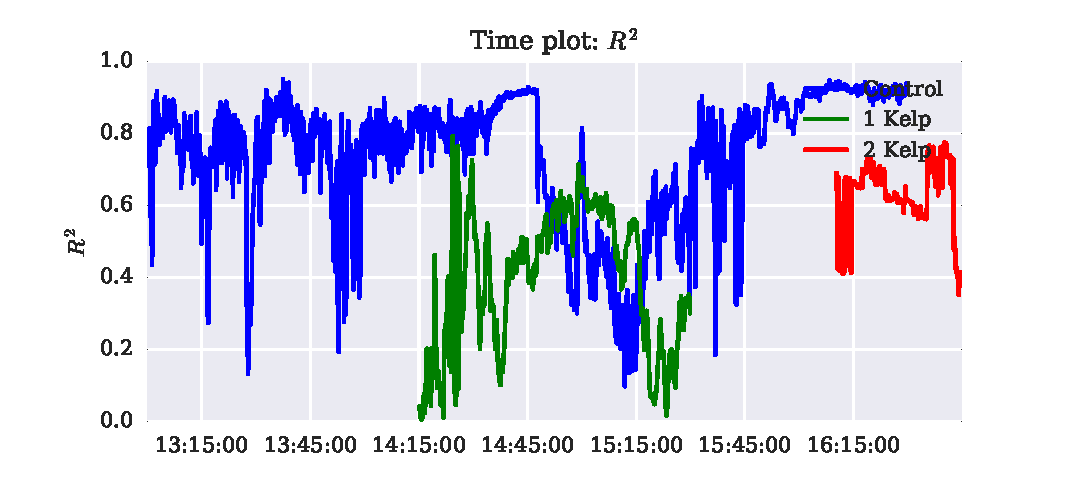
\includegraphics[width=\plotwidth]{time_r_squared.eps}
	\caption{$R^2$ over time}
	\label{time_r_squared}
\end{figure}

\subsubsection{Attenuation Coefficient Distribution}
The distributions of $k$ is shown using both bar plots and kernel density estimates (KDEs), in which each data point is represented by an exponential function of width similar to the bin width of the histogram, and the normalized sum of the exponentials is drawn to continuously represent the distribution.

\begin{figure}[H]
	\centering
	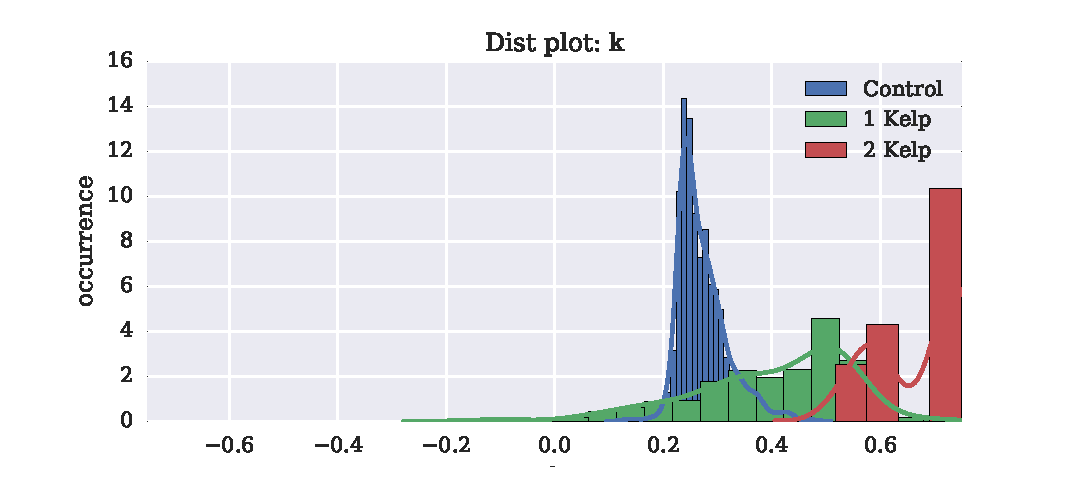
\includegraphics[width=\plotwidth]{dist_k.eps}
	\caption{Distribution of fitted values for attenuation coefficient}
\end{figure}

\subsubsection{Joint Plots}

The distributions of $k$ and $I_0$ are plotted together. In the first following figure, all three datasets are plotted together. In the following three plots, $k$ and $I_0$ are plotted using individual (1d) KDEs on the side and top, and a joint (2D) KDE represented by a contour plot in the center.

\begin{figure}[H]
	\centering
	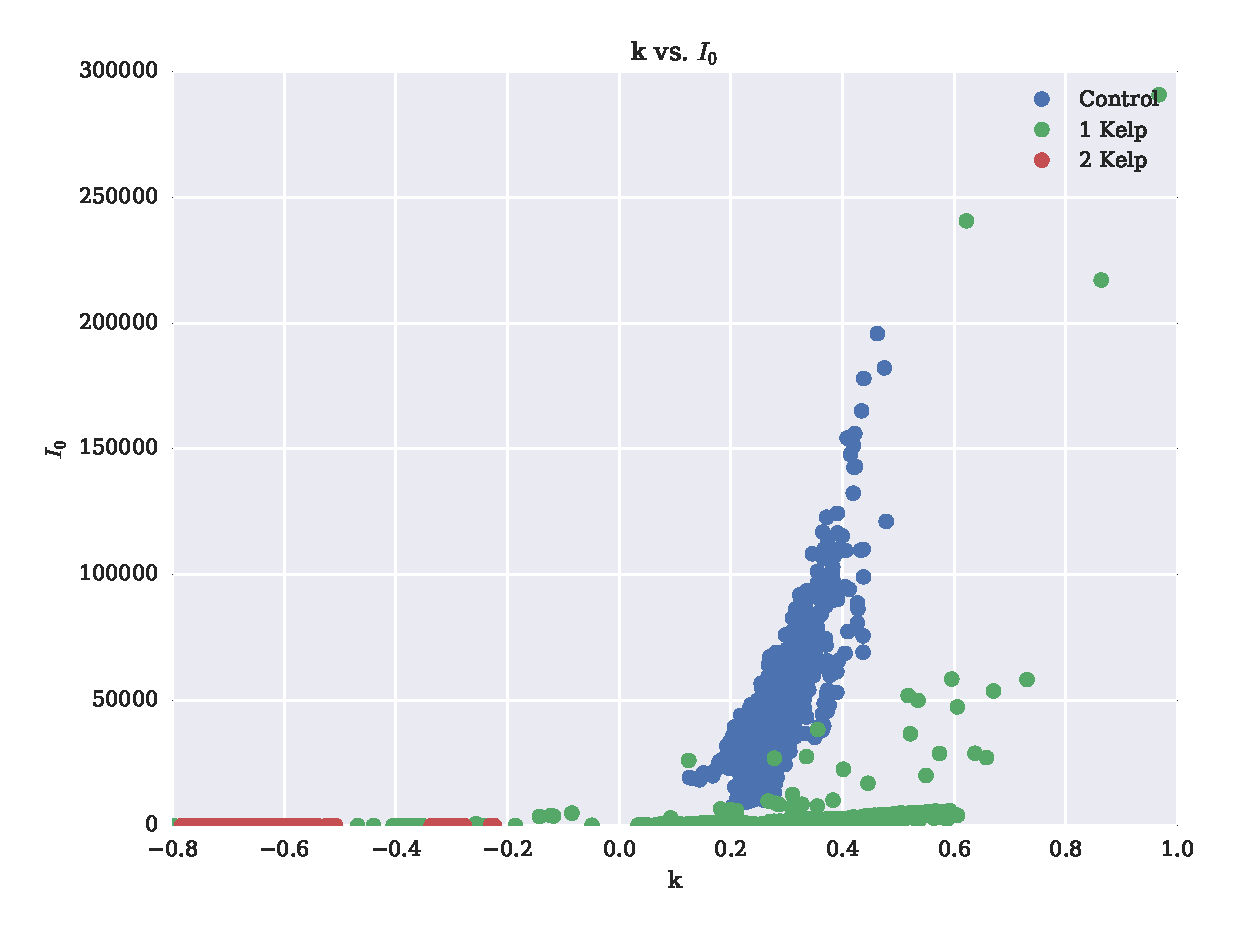
\includegraphics[width=\textwidth]{k_I0.eps}
	\caption{Joint distribution of $k$ and $I_0$ for all datasets}
\end{figure}

\begin{figure}[H]
	\centering
	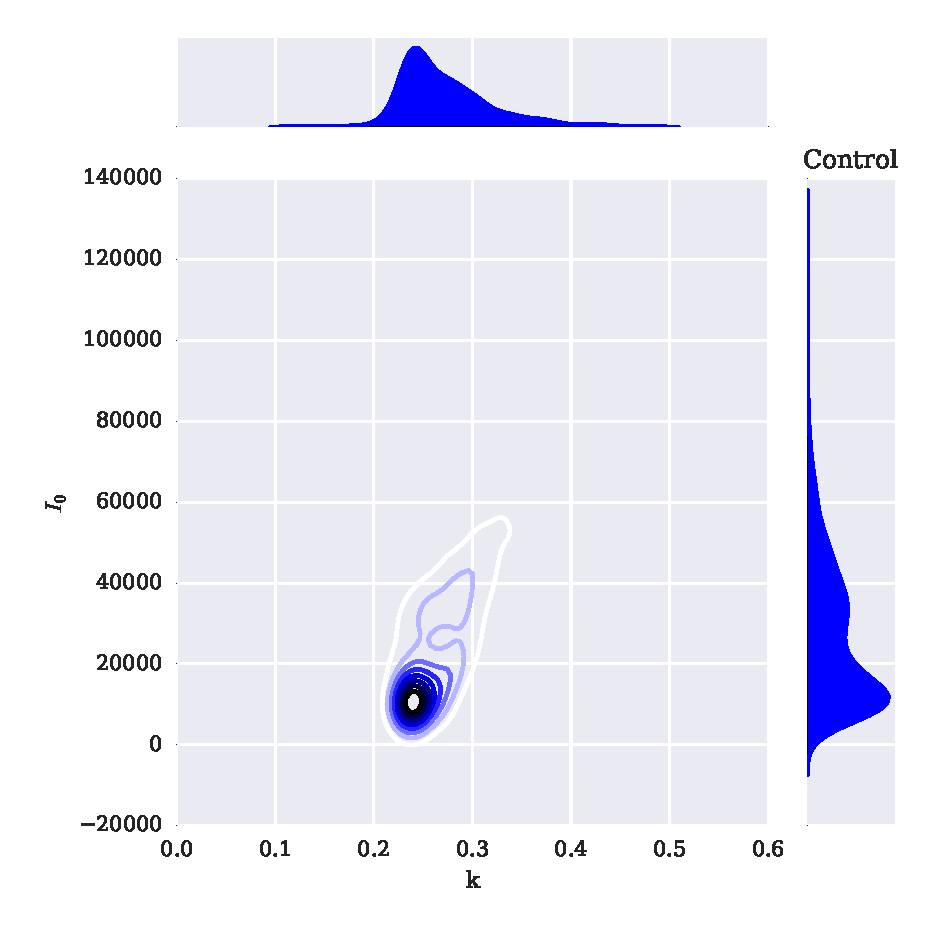
\includegraphics[width=\textwidth]{joint_control.eps}
	\caption{Joint distribution of $k$ and $I_0$ for \textbf{Control}}
	\label{joint_control}
\end{figure}

\begin{figure}[H]
	\centering
	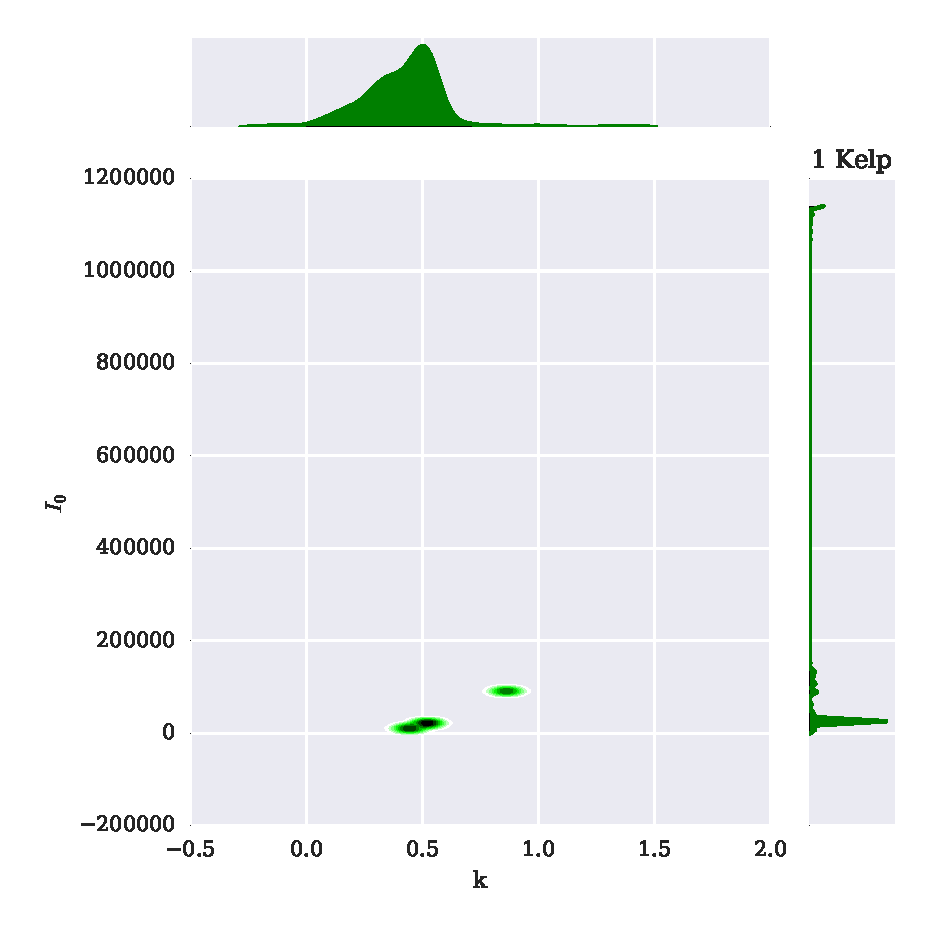
\includegraphics[width=\textwidth]{joint_1_kelp.eps}
	\caption{Joint distribution of $k$ and $I_0$ for \textbf{1 Kelp}}
	\label{joint_1_kelp}
\end{figure}

\begin{figure}[H]
	\centering
	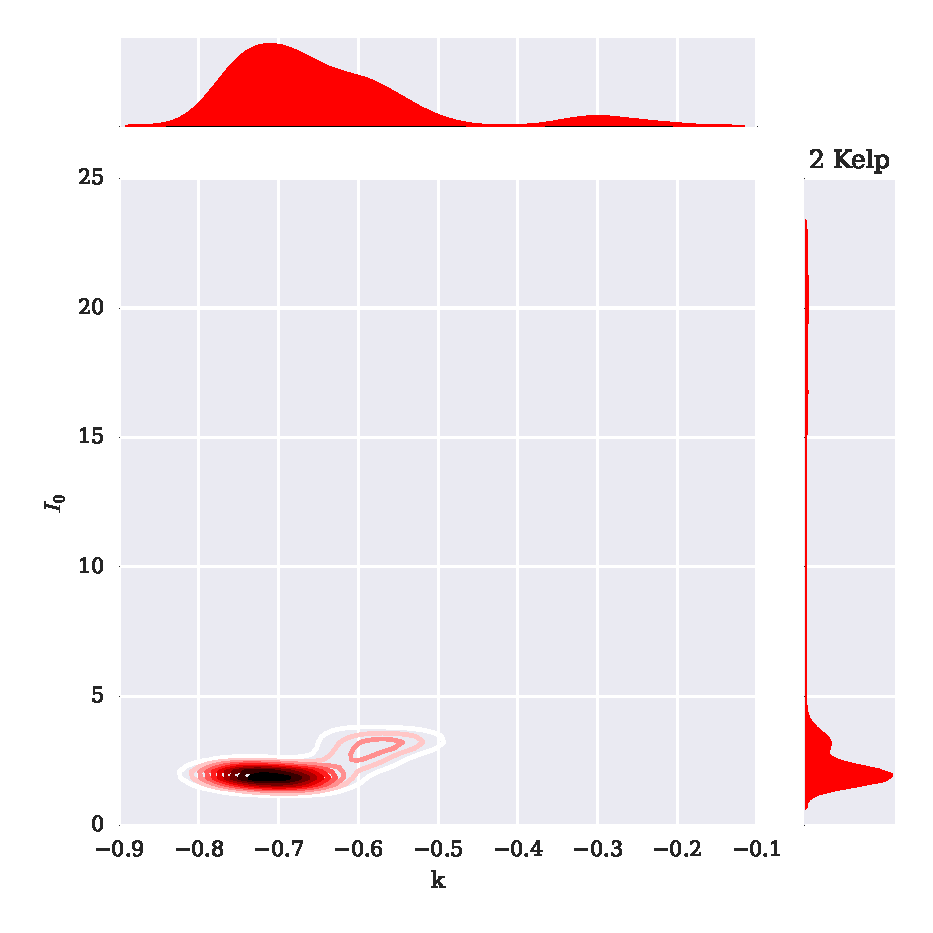
\includegraphics[width=\textwidth]{joint_2_kelp.eps}
	\caption{Joint distribution of $k$ and $I_0$ for \textbf{2 Kelp}}
	\label{joint_2_kelp}
\end{figure}

\subsection{Interpretation}
As is evident from the plots, all of the data is very noisy. The data does not fit the model perfectly, although in some cases the model is fairly successful. In particular, the attenuation measured by the sensors on the rope without kelp fits the model quite well, as can be seen by the relatively constant value for $k$ in figure \ref{time_k}, as well as by the small standard deviation shown in figure \ref{stats_control}. The model was fairly successful for the rope with 1 kelp plant. The data is certainly noisier than the control data. In figure \ref{joint_2_kelp}, it can be seen that the joint KDE for $k$ and $I_0$ seems to have 2 local maxima, which is symptomatic of a lack of consistency in the fitting. For the rope with 2 kelp plants, though, the analysis did not produce clear results. As is shown in the figures and the statistical table, negative values of $k$ are calculated. This would imply that light intensity is increasing with depth. Furthermore, the raw intensities as well as the calculated values for $I_0$ are several orders of magnitude lower than in the other cases. It is not clear why this is the case. Some possible cases are:
\begin{itemize}
	\item Kelp density varies with depth, so perhaps there is more kelp towards the surface than there is near the bottom of the rope.
	\item We are using the wrong time frame for this dataset. Perhaps the experiment with 2 kelp plants actually occurred at a different point during the day than the section being considered.
	\item The rope was placed in the water upside down. This could explain both the increasing intensity and lower magnitudes.
	\item Some unknown event was disrupting the experiment, e.g. large waves, fish, other boats, etc.
\end{itemize}

We will repeat the experiment on June 11th. Similar analysis will be performed with the new data, and the results will be compared.